%!TEX root = ../main.tex

We illustrate how \jilette can be used to run symbolic tests for \emph{unspecified} JavaScript code 
and to automatically generate symbolic tests for JavaScript code annotated with separation logic specifications. 
To this end, we make use the JavaScript implementation 
of a  \emph{key-value map} given in Figure~\ref{map:example}~(left). 
This implementation contains four functions: 
\jsinline|Map|, for constructing an empty map;
\jsinline|get|, for retrieving the value associated with the key given as input;
\jsinline|put|, for inserting a new \emph{key-value pair} into the map and updating the values of existing keys; and
\jsinline|validKey|, for deciding whether a key is valid.

\myparagraph{Prototype chains and $\mathtt{Object.prototype}$}
In order to better understand the implementation of the map library as well as its possible bugs, 
one must first understand the \emph{prototype-based inheritance} mechanism of JavaScript. 
Every JavaScript object has a prototype, which (for presentation purposes) we assume to 
be stored  in an internal property \jsinline|@proto|. In order to determine the value of a property
\jsinline|p| of an object \jsinline|o|, the semantics first checks if \jsinline|o| has a 
property named \jsinline|p|, in which case the property look-up yields its value. Otherwise, the 
semantics checks if \jsinline|p| belongs to the properties of the prototype of \jsinline|o| and so 
forth. Hence, in the example, when looking up the value of the property \jsinline|hasOwnProperty|
of the object \jsinline|contents|, one gets the value associated with the property  \jsinline|hasOwnProperty|
of its prototype.
The sequence of objects that can be accessed from a given object through the inspection 
of the respective prototypes is called a \emph{prototype chain}.
Prototype chains typically finish with the object \jsinline|Object.prototype| from which JavaScript 
programs can access a number of built-in functions, which are part of the language runtime environment and are used for inspecting and manipulating objects.
An example of such a function is \jsinline|hasOwnProperty(p)|, which checks whether or not the object 
on which it is invoked has the property \jsinline|p| (e.g. {\small \jsinline|map.hasOwnProperty("_contents")|}
evaluates to \jsinline|true| when evaluated in the heap shown in Fig.~\ref{map:example}-(right), 
because the object \jsinline|map| has a property named~\jsinline|"_contents"|). 

\myparagraph{Description of the example}
The map library implements a \emph{key-value map} as an object with property \jsinline|_contents|, denoting the object storing the map contents.  
The named properties of \jsinline|_contents| and their value attributes correspond to the map keys and values, respectively.
The functions \jsinline|get|, \jsinline|put|, and \jsinline|validKey| are to be shared between all map 
objects. Therefore, they are defined in \jsinline|Map.prototype|, which is the prototype 
of all objects created using \jsinline|Map| as a constructor (i.e.~using~\jsinline|new Map()|).

 \begin{figure}[t!]
 \begin{minipage}{0.5\textwidth}
 \begin{lstjs}[firstnumber=1]
function Map () { this._contents = {} }

Map.prototype.get = function (k) {
  var c = this._contents;
  if (c.hasOwnProperty(k)) {
    return this._contents[k] 
  } else { return null }
}

Map.prototype.put = function (k, v) {
  var c = this._contents;
  if this._contents.validKey(k)) {  
    contents[k] = v   
  } else
    throw new Error("Invalid Key");
} 

Map.prototype.validKey = function (k) { ... }
\end{lstjs}
\end{minipage}
\ 
 \begin{minipage}{0.4\textwidth}
 \hspace*{-1.2cm}
 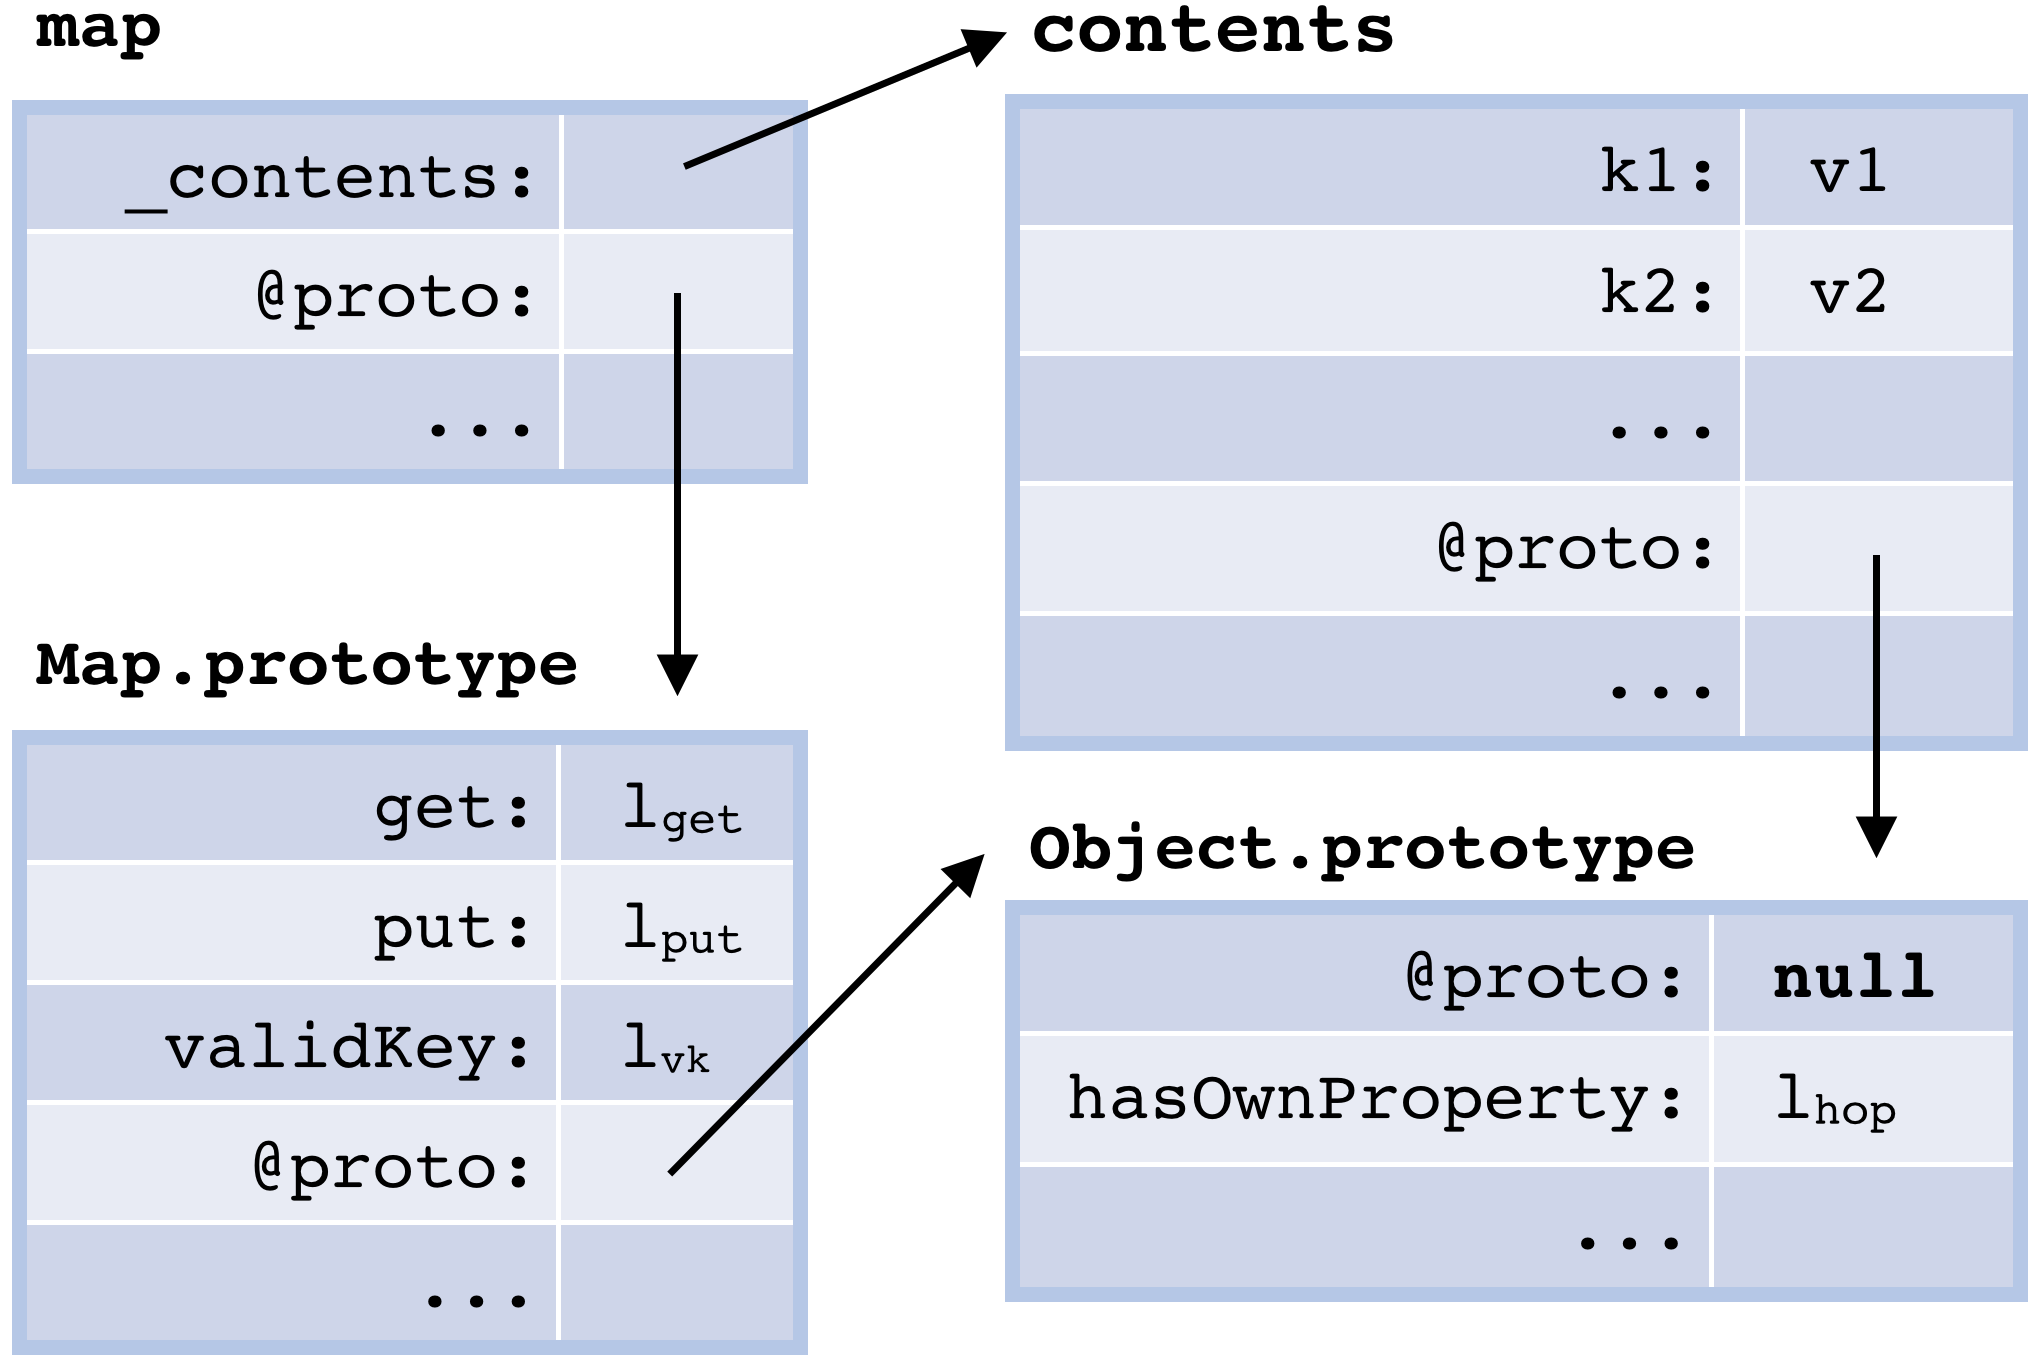
\includegraphics[width=1\textwidth]{figures/mapDiagram.png}
 \end{minipage}
\caption{JS map implementation (left) and example of a map library heap (right) \label{map:example}}
\end{figure}

\lstnewenvironment{lstjsex}{\lstset{language=JavaScript,basicstyle=\fontsize{8}{8}\ttfamily,escapeinside={~}{~}, numbers=none, backgroundcolor=\color{mygray}}}{}


\subsection{Symbolic Testing}

A simple way of testing the behaviour of the key-value map is to write a 
 
%
Note that one can insert a key-value pair with \jsinline|"hasOwnProperty"| as a key into the map. 
By doing this, \jsinline|"hasOwnProperty"| in the prototype chain of
\jsinline|_contents| is overridden and subsequent calls to \jsinline|get| will fail. 
Consider the following symbolic test:
\begin{lstjsex}
var s1 = __s(); var n1 = __n(); 
var m = new Map();  m.put(s1, n1); var r = m.get(s1);  
assert(n1 = r)
\end{lstjsex}
%
The symbolic test above checks for a desired property of the library---if we were to put a key/value pair \jsinline|(k, v)| into the map, then we should be able to retrieve the value \jsinline|v| using the key \jsinline|k|. We can run \jilette on this test to reveal the bug discusses above. Indeed, \jilette generates
the failing model: \jsinline|s1 = "hasOwnProperty"|. 

This example also highlights how \jilette does not require 
specialist knowledge, and can, therefore, be used by almost any JavaScript developer. 
The annotation burden amounts to the creation of symbolic variables and the writing of assertions, remaining minimal and intuitive, in stark contrast with the standard annotation 
burden of verification tools.




